\section{Skill Compilation}
\label{sec:compiler}

When a user installs a skill for the first time, \sys compiles it against the target (model, harness, host environment) before the skill ever runs.
The compiler reads the raw skill text, identifies the target,
and produces one or more optimized \emph{skill variants} through three sequential passes.
Each pass closes a different kind of gap between what the skill expects and what the target provides.

\subsection{Capability-Based Compilation}
\label{sec:compiler:cap}

The first pass addresses the model and harness mismatch.
Because targets vary widely (\S\ref{sec:insight:challenges}),
the compiler cannot embed optimization logic specific to each target.
Instead, \sys introduces \emph{primitive capabilities},
an abstract vocabulary for expressing what a skill requires and what a target can provide.
The compiler profiles each target offline with microbenchmarks for these capabilities,
compares the profiling result with the skill's capability requirements,
and selects the optimization strategy based on the gap.

\subsubsection{Primitive Capabilities}

Just as JVM bytecodes define the basic operations a Java program requires from its runtime,
primitive capabilities define the basic abilities a skill requires from its target.
A primitive capability is an indivisible unit that describes what is needed to complete the tasks a skill defines.
It is defined purely from the demand side, independent of any specific model.
The definition of primitive capabilities follows three principles:
\begin{myitemize}
  \item \emph{Composability}: any concrete task within a skill can
    be described as a combination of primitive capabilities.
  \item \emph{Generality}: each primitive capability must be broad
    enough to appear across many skills, keeping the total
    capability set small and the compiler's workload bounded.
  \item \emph{Semantic independence}: a primitive capability concerns structural correctness,
  rather than whether the output is insightful or well-argued.
\end{myitemize}

We derived the primitive capability set from a corpus of 15,063 skills
in two stages. First, we curated 50 representative skills spanning
document generation, script execution, data analysis, and code
development, and used LLM-assisted analysis guided by the three
principles above to decompose them into an initial set of 19
primitive capabilities. We then manually reviewed each primitive capability to verify that
it satisfies all three principles. Second, we validated the initial
set against the full corpus of 15,063 skills by checking whether
each skill's requirements can be expressed as a combination of the
existing primitives. Skills that could not be covered revealed
missing capabilities. A missing capability was added to the set only
when it appeared in at least 1\% of the corpus, filtering out
rare or domain-specific requirements. This process converged on
26 primitive capabilities across four categories that cover the
requirements of 95\% of the skills.

We also observe that different tasks demand the same
primitive capability at different depths. We therefore
define multiple proficiency levels for each primitive capability.
A higher level represents deeper use of the capability: an \emph{L(n+1)} requirement
cannot be satisfied by \emph{L(n)} ability.
Table~\ref{tab:primitives} shows representative examples.
For each primitive capability level, we generate a suite of microbenchmarks
and evaluate them across different models.
If a model succeeds on higher-level microbenchmarks while failing on lower-level ones,
we interpret this inconsistency as evidence that the level hierarchy is miscalibrated.
We then revise the level definitions and repeat the evaluation.

\begin{table}[t]
\setlength{\abovecaptionskip}{4pt}
\setlength{\belowcaptionskip}{0pt}
\centering
\caption{Representative primitive capabilities and their
  proficiency levels. The full catalog contains 26 primitive capabilities
  across four categories.}
\label{tab:primitives}
\resizebox{\columnwidth}{!}{%
\begin{tabular}{@{}llll@{}}
\toprule
\textbf{Primitive} &
  \textbf{L1} & \textbf{L2} & \textbf{L3} \\
\midrule
gen.code.shell &
  Basic commands (ls, cat) &
  Pipes, redirection, loops &
  Complex pipelines (sed, awk) \\
\addlinespace
reason.arithmetic &
  Single-step ops &
  Multi-step &
  Compound \\
\addlinespace
tool.exec &
  Single command &
  Params and relative paths &
  Chained multi-step execution \\
\addlinespace
follow.procedure &
  3 sequential steps &
  5--7 with branches &
  Loops and verification \\
\bottomrule
\end{tabular}%
}
\end{table}

\subsubsection{Measuring the Gap Between Skill and Target}

Before applying optimizations, the compiler must determine
the gap between what the skill requires and what the target
provides. On the skill side, the compiler extracts the
skill's capability requirements at install time: it
decomposes the skill into concrete tasks and maps each task
to the primitive capabilities it requires. 

On the target side, \sys profiles the target with
microbenchmarks generated for each primitive capability to
measure how well the target supports it.
Success on a microbenchmark for a primitive capability at a given level
indicates that the model has attained at least that level of proficiency for that capability.
This profiling is performed when the user sets up the agent and model.
The results are cached and reused for all skill compilations
for the same target.

\subsubsection{Capability-Aware Skill Transforms}

With the skill's capability requirements and target's capability profile in hand, the compiler
walks through each capability requirement and selects a
transform based on the gap between the required level and
the target's profiled level.

\textbf{\emph{Compensation}} applies when the target supports the
required capability but at a lower level.
The compiler first identifies the distinctions between the two levels of a primitive capability.
It then transforms the skill accordingly to reduce its capability requirement from a higher level to one supported by the target model.
Such transformations may include providing examples, making instructions more explicit, and strengthening task constraints.
Compensation is the preferred transform because it preserves the skill's original intent.

\textbf{\emph{Substitution}} is the fallback when compensation is
not viable: the target lacks the capability entirely, or the
level gap is too large for compensation to bridge reliably.
The compiler switches to an alternative
implementation path that achieves the same goal using
different capabilities. For example, if a skill requires
gen.code.python at L3 for a pandas workflow but the target
only reaches L1, the compiler can switch to an SQL-based
path if the target's gen.code.sql reaches L2. These
alternative paths form \emph{equivalence classes} that the
compiler identifies during requirement extraction.

\begin{figure}[t]
  \centering
  \setlength{\abovecaptionskip}{5pt}
  \setlength{\belowcaptionskip}{0pt}
  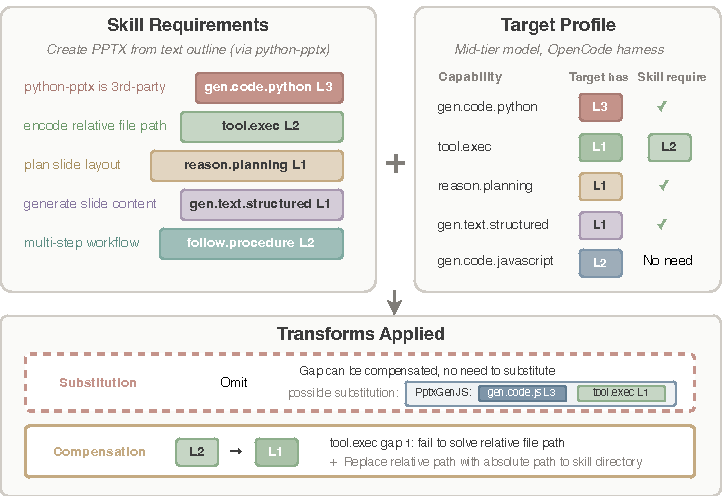
\includegraphics[width=\columnwidth]{figures/compilation-case-study.pdf}
  \caption{Capability-based compilation on a PPTX skill.
    The compiler extracts skill requirements (left),
    profiles the target (middle), and applies transforms
    based on the gap (bottom).}
  \label{fig:compilation_case}
\end{figure}

\heading{Case Study.}
Figure~\ref{fig:compilation_case} illustrates the
compilation process on a real skill that teaches an agent
to create PPTX presentations using python-pptx.
The skill requires five primitive capabilities at varying levels.
The target matches four of them directly but provides
tool.exec at only L1, while the skill requires L2 for
resolving relative file paths.

The compiler identifies a possible substitution path:
switching to \emph{PptxGenJS} via \emph{gen.code.javascript} would replace
python-pptx and lower the tool.exec requirement to L1.
However, because the tool.exec gap is only one level,
compensation is preferred. The L2 profiling results reveal
that this model fails to resolve relative file paths when
executing commands. The compiler injects absolute path
resolution into the compiled skill, replacing relative paths
with absolute paths to the skill directory.

\begin{figure*}[t]
  \centering
  \setlength{\abovecaptionskip}{3pt}
  \setlength{\belowcaptionskip}{0pt}
  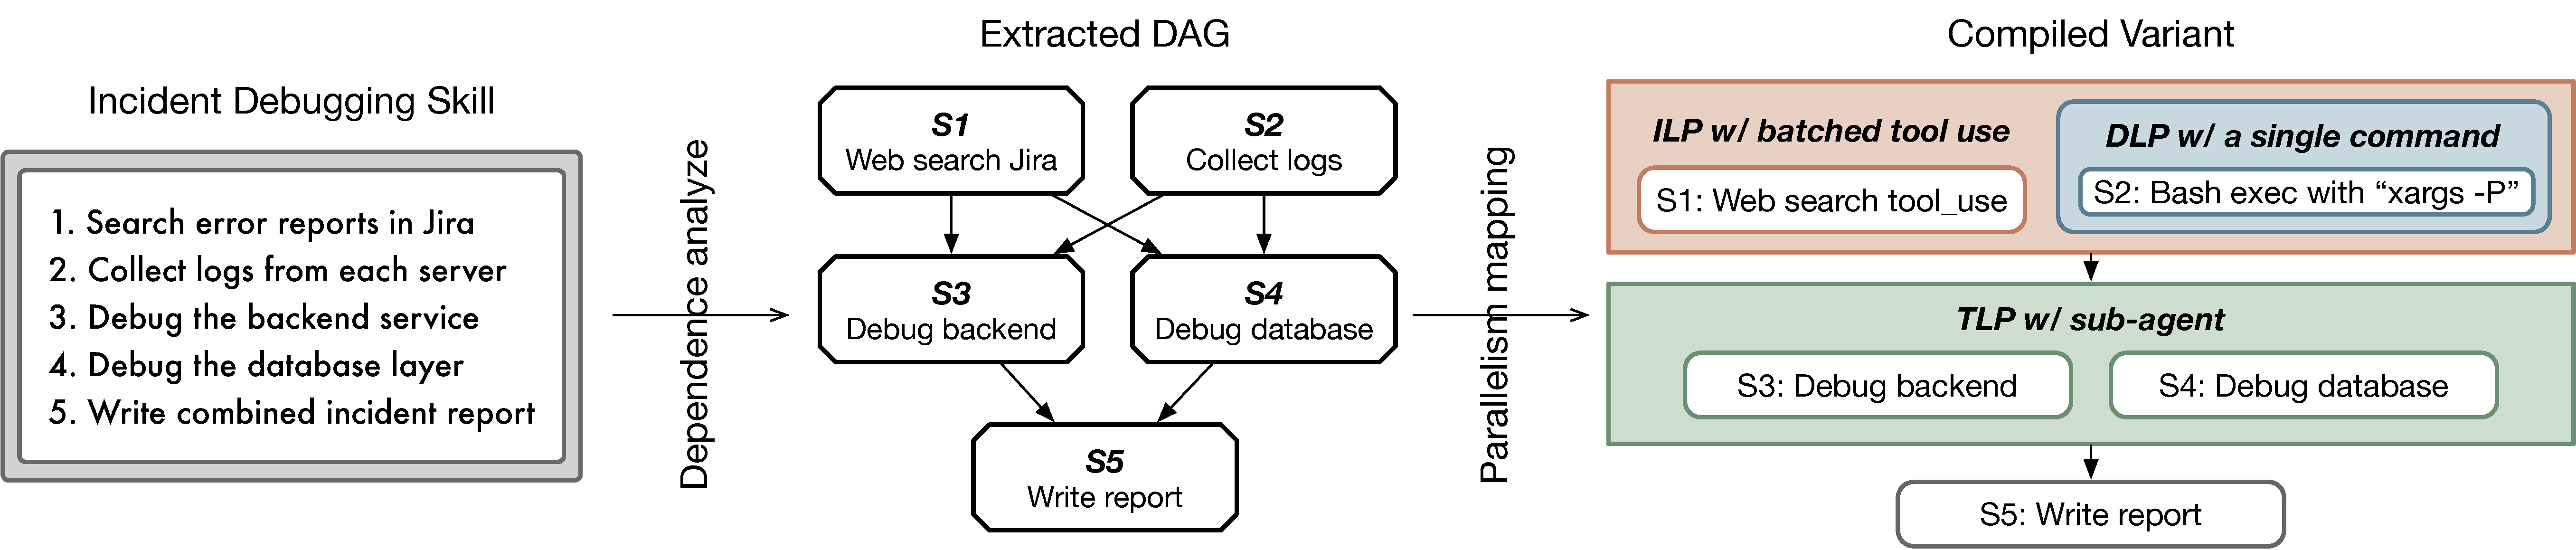
\includegraphics[width=\textwidth]{figures/concurrency_extraction.pdf}
  \caption{Concurrency extraction on an incident-response skill.
    The compiler decomposes sequential steps into a workflow DAG,
    identifies parallel opportunities both between steps and within
    steps, and maps each to the appropriate concurrency primitive.}
  \label{fig:concurrency_extraction}
\end{figure*}

\subsection{Environment Binding}
\label{sec:compiler:env}

The second pass resolves \emph{P3: environment mismatch}.
Rather than merely checking whether dependencies are installed,
the compiler uses a built-in \emph{env-binding skill} to
reconcile the skill's assumptions against the host environment and
generate an env-binding script.

At skill installation time, the compiler first extracts a dependency manifest from the output
skill of the first pass and any explicit prerequisites, covering external libraries, CLI tools, and system services.
For each manifest entry, the compiler runs a lightweight presence check (e.g., pip show, which).
Dependencies that are already satisfied require no further work.
When the check fails, the compiler performs deeper, system-aware probing to
determine how to resolve the dependency.
The compiler then emits an idempotent env-binding script which will check and repair the dependency before skill execution.
When the environment changes or the env-binding script fails,
execution falls back to the model, and the script's output is passed to the model as additional context.

\subsection{Concurrency Extraction}
\label{sec:compiler:par}

The third pass finds parallelism hiding in plain sight.
Recall that 76\% of skills contain procedural structure
(\S\ref{sec:insight:analysis}). These skills describe
multi-step workflows in sequential prose, but not every step
actually depends on the one before it.

The compiler uses LLM-assisted analysis to decompose the
skill into discrete steps, identifying for each step what
inputs it consumes and what outputs it produces. It then
builds a workflow DAG: nodes are steps, and an edge from
step A to step B exists when B consumes an output of A.
The compiler also analyzes each step internally for
sub-operations that can proceed concurrently.
Figure~\ref{fig:concurrency_extraction} illustrates this
process on an incident-response skill.
For each parallel opportunity, whether between steps or within a
step, the compiler selects a concurrency primitive based
on the task structure and the harness. \sys defines three
levels of parallelism.

\myparagraph{Data-Level Parallelism (DLP).}
A single step applies the same operation to multiple
independent data items, such as running the same analysis
on each of 15 CSV files. The compiler rewrites the step to
process items concurrently using language-level parallelism
primitives appropriate to the skill's implementation, such
as shell-level parallel execution, Python's multiprocessing,
or JavaScript's Promise.all. DLP requires no special
harness support.

\myparagraph{Instruction-Level Parallelism (ILP).}
Multiple independent steps each need a tool call with no
data dependency between them, such as running eight
independent code-analysis scripts on a project. The compiler
groups the corresponding DAG nodes into one parallel stage
and rewrites the skill so that their tool invocations are
issued together in a single LLM turn, instead of one after
another in sequential prose. The compiler annotates the skill with which
step outputs should be bound back to which downstream DAG
inputs after the batch completes. ILP requires the
harness to support batch tool dispatch.

\myparagraph{Thread-Level Parallelism (TLP).}
The workflow decomposes into independent sub-tasks that each
require multi-turn reasoning, such as debugging three
independent services. The compiler rewrites the skill to
extract each sub-task into a separate sub-agent block with
an explicit task description, declared input context, and
expected output that can be consumed by the parent workflow.
The annotation marks this block for sub-agent dispatch, so
the runtime spawns one sub-agent per block in its own
session and merges the returned outputs back into the DAG.
TLP requires harness support for sub-agent spawning.

Opportunities whose required primitive is unavailable on the
target harness fall back to sequential execution.
For each viable opportunity, the compiler either rewrites
the skill's instructions to execute items concurrently (DLP)
or emits execution annotations that make the parallel
structure explicit: a parallel stage over DAG nodes for ILP
or a sub-agent task block with input and output contracts
for TLP. The runtime reads these annotations and dispatches
them with the corresponding harness primitive.
